\chapter{Misura della velocità della luce}

L'obiettivo del nostro esperimento è misurare la velocità della luce $c$.

L'apparato di misurazione consiste principalmente in:
\begin{itemize}
 \item Un laser Elio-Neon ($\lambda=32$ nm).
 \item Uno specchio rotante a velocità angolare regolabile.
 \item Due lenti convergenti, di lunghezza focale $l_1 = 48mm$ e $l_2 = 252 mm$.
 \item Un microscopio con beam splitter e micrometro.
\end{itemize}

Lo specchio rotante viene fatto girare con velocità angolare $\omega_1$ in senso orario e $\omega_2$ in senso antiorario. Queste velocità angolari sono identiche nella maggior parte dei casi, e la loro differenza è trascurabile.

Chiamando $s_{cw}$ e $s_{ccw}$ rispettivamente le misure con specchio rotante in senso orario e antiorario, per come è orientata la strumentazione il numero
$$\Delta s = s_{cw} - s_{ccw}$$
deve essere positivo.

Purtroppo però non è questo il caso per qualche misura presa in mattinata, per ragioni sconosciute e che non siamo riusciti a riprodurre. Questi dati sono esclusi dalla misurazione in quanto evidenti errori, e sono mostrati in rosso nel grafico seguente
I dati sono molti, dunque forniamo qui soltanto una visione grafica, e lasciamo la tabella come allegato.

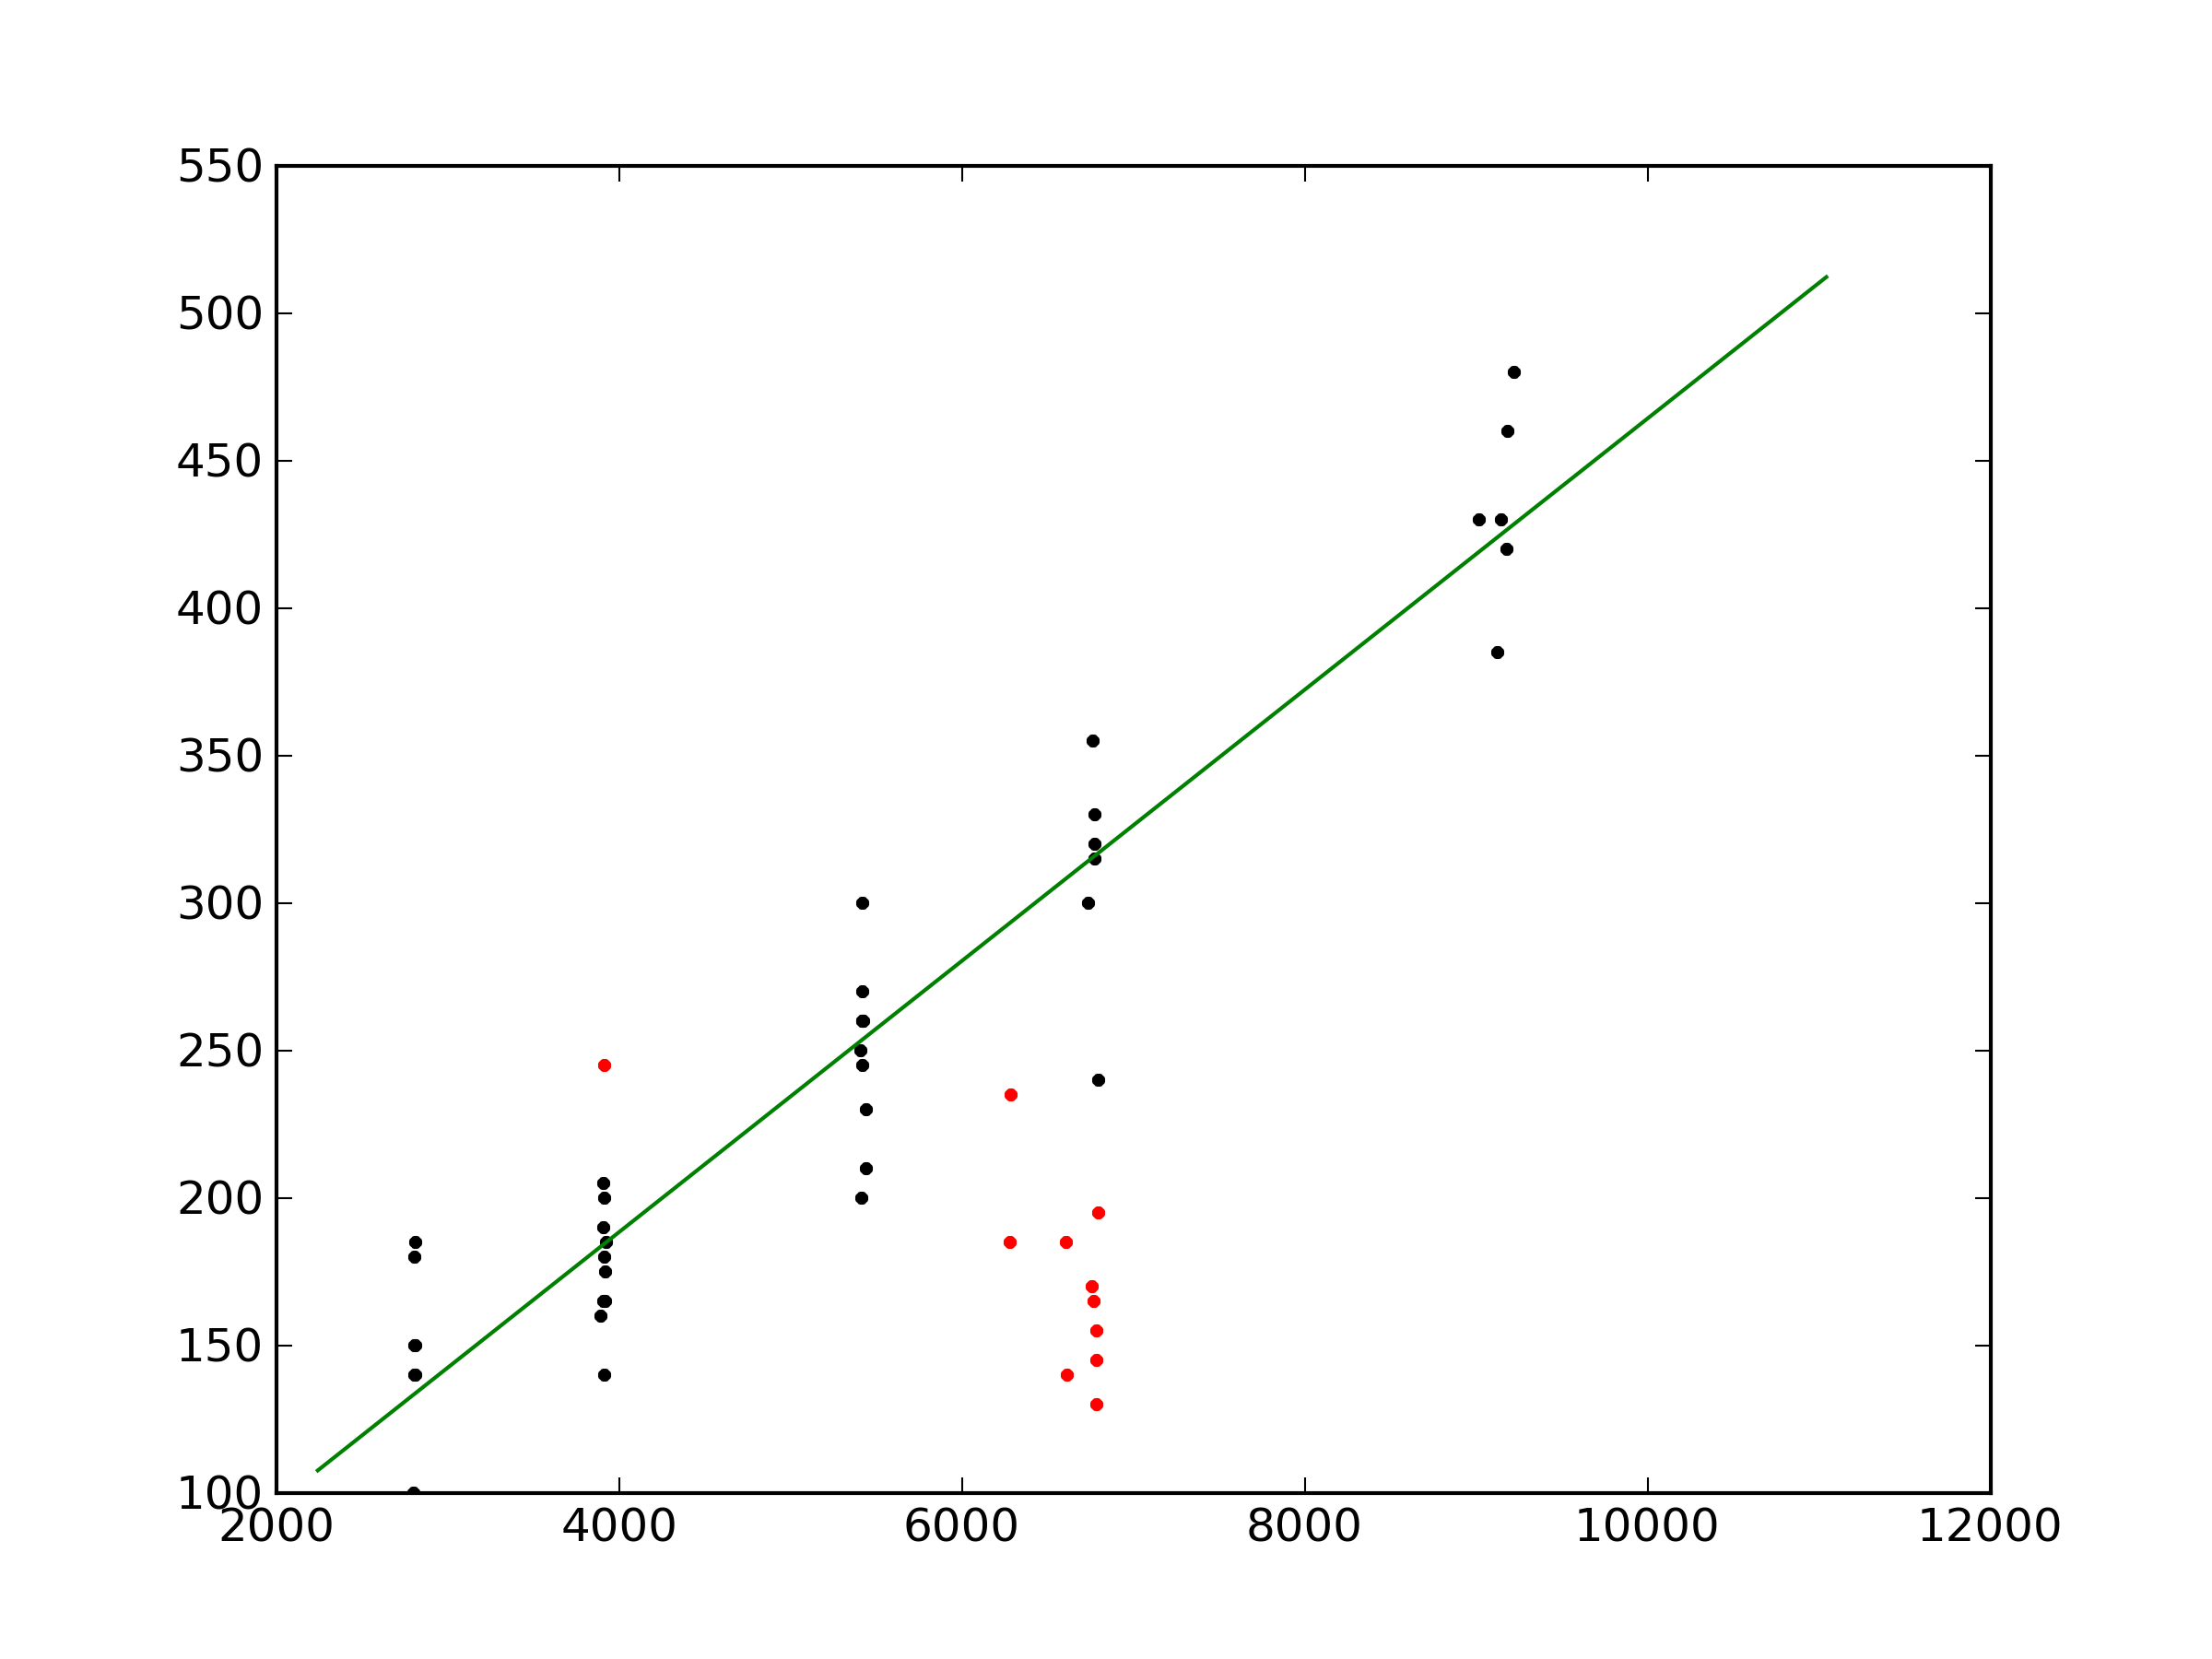
\includegraphics[scale=0.75]{grafici/C/dati.png}

\section{Analisi dati}

Chiamiamo $D = 13.480$m il cammino geometrico della luce per tornare allo specchio rotante, ovvero il doppio della distanza specchio rotante/specchio fisso; $A$ la distanza del punto di convergenza del fascio laser dalla lente $l_2$ e $B$ la distanza tra $l_2$ e lo specchio rotante. 

Per calcolare con precisione $A$, conoscendo la distanza focale di $l_2$, la ricaviamo dalla formula dei punti coniugati:
$$A=\frac{(B+D)f}{B+D-f} = 256\text{mm}$$


Per calcolare $c$, dobbiamo interpolare i dati presi nel modo seguente:
$$\Delta s = \frac{\tilde{A}}{c}\omega$$
ove
$$\tilde{A} = \frac{4*A*D^2}{2}$$

$\sage{2*e^2}$

La funzione che ci permetterà di calcolare $c$ è la seguente:

$$c = \frac{\tilde{A}}{m}$$
ove

Data una 
m=0.04594423946498933

Ricaviamo, tramite  il fit della funzione $V=R*I$" dove R è parametro da stimare, due resistenze ignote.


Misuro la resistenza interna del voltometro, mantenendo costante la ddp a $14.5\ V$ e variando la resistenza all'interno del circuito. 
Il voltmetro è in parallelo al circuito, perciò $R_i$:

$$R_i = \frac{RV}{RI-V} $$

dove R è la resistenza variabile, I la corrente nel circuito e $V= 14.5\ V$


La resistenza risulta $9.20 \pm 0.27 \ M \Omega$.


Misuriamo la resistenza interna dell'amperometro, che è collegato in serie al circuito. 

$$R_i = \frac{V-RI}{I}$$

In questo caso, R è fissato ($R=0.5 \Omega$) e sono V e I a variare

La resistenza interna risulta $11.42 \pm 0.45 \Omega$



Colleghiamo una piccola lampada a filamento al circuito, e verifichiamo che il suo comportamento resistivo non segue la legge di Ohm. 





